\chapter{框架扩展}
\label{cha:ext}

\section{引言}%1.5
基于“生成-检验”框架的程序自动修复系统以源代码和其对应的测试用例为输入,输出一组能够使测试集中所有测试用例通过的程序变体供开发人员参考。从设计的目标来看,“生成-检验”系统希望能够接手开发人员的调试工作,提高软件开发效率。然而从实验数据来看,现有系统在修复规模稍大的程序时速度仍然比较慢。例如,SPR在实验对象程序php上常常需要几个小时才能完成修复,我们实现的系统PFDebug在修复Closure Compiler上的错误时也要花费几个小时。
另一方面,由于系统中搜索引擎能够在有限时间内搜索完的搜索空间有限,现有系统一般只能在单一位置生成如表达式替换、方法替换等比较简单的修改方案,导致现有系统的修复正确率也不太高,例如SPR在GenProg的测试集上修复了39/69个错误,PFDebug修复了24/357个错误。由于速度慢、正确率低,基于“生成-检验”框架的自动修复系统与实际应用仍有一定的距离。

从使用者的角度,遵循“生成-检验”框架开发的系统在计算过程中间不需要开发人员的参与,也不需要了解程序错误相关的更多信息。这一特点使得系统使用非常方便——只要启动程序,等待结果就可以了。但是,考虑到现有自动调试技术的发展水平,这种模式未必是“生成-检验”系统的最佳利用方式。事实上,如果能够让开发人员与系统有一定的互动,充分利用开发人员的调试经验、对调试任务的理解、错误类型的初步判断等信息,系统的修复速度可能得到进一步的提高,搜索空间也可以更大,正确率也随之提高。

基于上述想法,本章提出扩展“生成-检验”框架,使系统能够与开发人员充分共享信息,优化修复效果。扩展方式有两种,第一种是“交互式调试”,基本思想是,利用开发人员对程序的理解,向开发人员提供接口描述他对程序运行状态的判断,使系统能够将错误限定于较窄的范围内,提高错误定位的准确度。此外,系统允许开发人员将调试任务分为几个小任务逐个解决,这使得系统可以处理需要在多个位置修改才能完成的调试任务。第二种是针对单类别错误修复的可扩展框架,即规范“生成-检验”框架的基本结构,使得错误定位方法易于替换,搜索空间易于剪裁,方便在此系统上进行二次开发,形成针对特定错误类型的修复系统。

为验证框架扩展的有效性,本章首先在已有框架上实现了“交互式调试”使用模式,形成了新的系统SmartDebug,并以多个实际程序为调试对象比较使用SmartDebug和人工调试的调试效率。实验表明,使用SmartDebug确实加速了调试任务完成过程。此外,本章整理了已有系统的框架结构,设计了方便扩展的开放接口,并在此框架上实现了针对空指针异常(NullPointerException)的修复系统。我们在CWE\_NullPointerDereference测试集上进行试验,成功修复了测试集中6个子类错误中的5个子类。

本章的主要贡献如下:
\begin{itemize}
	\item 提出“交互调试”扩展方式并实现,形成新的系统SmartDebug。在一组真实程序上进行实验,结果表明SmartDebug能够加速开发人员完成调试任务的过程
	\item 提出将现有系统扩展为针对特定类别错误修复系统的扩展方式,并给出开放接口定义,将现有系统重构为可扩展框架xDebug
	\item 在xDebug框架内实现针对Java空指针异常的修复系统NPEDebug,并在CWE\_NullPointerDereference测试集上完成实验,成功修复其中6个子类错误中的5个子类,证实xDebug的可用性
\end{itemize}

\section{交互式调试}%8
\subsection{概述}%0.5

“交互式调试”是指在利用自动修复系统完成调试任务的过程中,开发人员可以通过特定方式向系统提供信息,影响系统计算过程的一种设计模式。现有的“生成-检验”框架不依赖开发人员对程序的先验判断,这使得系统虽然使用简单,但也由于没有人工指导常常花费许多时间生成和检验无效的修复方案。在本节我们给出“生成-检验”框架的一种扩展方式,使得开发人员可以方便地输入他对程序运行状态的期望及是否正确的判断,而系统能够根据这些信息缩减搜索空间、分解调试任务、提高运行效率。

具体而言,我们首先在“生成-检验”框架中引入“检查点”概念。“检查点”在程序执行过程中某一具体位置上的一个标记点。在工具使用者的角度,开发人员可以自定义检查点,同时附上对该位置上程序运行状态的判断,包括“程序是否运行正确”,“如不正确,运行状态应当是什么样子”。而对于系统来说,由于检查点将程序的执行过程分成了多个段落,利用开发人员的判断,系统可以将程序错误位置缩小到其中的某一段或某几段上,将调试任务分解,降低难度。

实现“交互式调试”需解决两方面的问题,一是开发人员应如何输入检查点,而是系统应如何利用检查点上的信息优化搜索过程。本节我们将从这两方面阐述交互式调试框架扩展方式。

\subsection{相关工作}%1

将用户交互与调试工具相结合的工作可分为两大类。第一类是以辅助工具本身的功能为中心,引入开发人员的输入,使得辅助工具的性能更佳。例如,在文章\cite{IPSETFUL}中,作者将开发人员引入SFL算法错误定位的过程。作者将代码行的可疑程度分为“安全”,“敏感”和“危险”三个等级。这时,开发人员应人工检查标为“危险”的代码行,去除其中的错误。在此基础上,开发人员还应选择覆盖了“危险”和“敏感”代码行的测试用例,这些测试用例的执行过程和测试结果将作为下一轮SFL错误定位的输入。由于SFL算法在程序错误有多处时定位精度常常不稳定,将开发人员的判断引入错误代码行在迭代过程中逐步浮现,多处错误可逐个修改。类似的,文章\cite{hongyu-fl}要求开发人员对SFL算法给出的可疑代码行给出判断,标出正确的代码行,将其从可疑列表中剔除出去。这一反馈过程会使SFL的定位结果越来越精确。

另一个典型的研究工作是Microbat\cite{microbat}工具。该工具集成在Eclipse IDE中,其主要目的是引导开发人员的调试过程。对于一个出错的程序,Microbat记录开发人员使用跟踪调试时程序的执行轨迹,从程序运行状态和上下文中分析出跟踪的哪些步骤可能出错并提示给开发人员。开发人员则分析提示给出的调试步骤,反馈给工具这一步骤是否真的有错,工具则据此调整输出,给出新的提示。

第二类是针对特殊类型的程序为开发人员提供方便的调试辅助设施。例如,针对并发程序的“记录-重放”工具LEAP\cite{LEAP},ODR\cite{ODR},ORDER\cite{ORDER},PRES\cite{PRES},bbr\cite{bbr}等能够记录多线程程序的具体执行路径并稳定回放,这使得开发人员可以在一个确定的执行路径上完成程序调试,而避免了多线程程序运行过程的随机性。工具Sherlog\cite{Yuan:2010:SED:1736020.1736038}能够通过分析已部署程序的运行日志还原程序的执行过程。在还原过程中,当遇到不确定因素时,SherLog会自动产生日志记录语句,从而确认程序的真实还原路径,最终方便开发人员定位错误。此外,BigDebug\cite{bigdebug1}\cite{bigdebug2}为开发人员提供程序执行过程的记录、重放和可视化功能,使得开发人员在使用已有的断点调试、日志分析技术基础上更高效的修复程序错误。

在辅助调试类工具外,代码片段提示工具CodeHint\cite{Galenson:2014:CDI:2568225.2568250}也利用了用户输入信息逐步精化工具的输出结果。CodeHint的功能是根据用户的要求自动生成表达式。用户描述需求的方式有三种,一是限定表达式的语法类型,二是直接给定表达式的值,三是通过CodeHint定义的pdspec语法描述表达式应满足的一条性质。CodeHint在一定的搜索空间中查找合法的表达式,并根据用户需求过滤结果。在使用过程中,用户可以逐步精化对表达式的要求,CodeHint也会不断扩大搜索空间生成新的结果。这一交互过程使得CodeHint能够不断将搜索方向靠近用户的期望,优化搜索结果。

%TODO
%\cite{Mechtaev:2016:ASM:2884781.2884807}
%	author = {Mechtaev, Sergey and Yi, Jooyong and Roychoudhury, Abhik},
%	title = {Angelix: Scalable Multiline Program Patch Synthesis via Symbolic Analysis},
%	booktitle = {Proceedings of the 38th International Conference on Software Engineering},
%	series = {ICSE '16},

现有的研究工作尚未在“生成-检验”框架中引入用户交互。本文在此方向进行探索性的研究,也希望对其他研究人员带来一定的启发。

\subsection{交互模式}%1

将用户交互引入“生成-检验”系统,首先需要设计用户与系统的具体交互模式。图\ref{fig:interact-model}以一段示意代码展示了开发人员与系统合作完成调试任务的主要步骤。

\begin{figure}
	\centering
	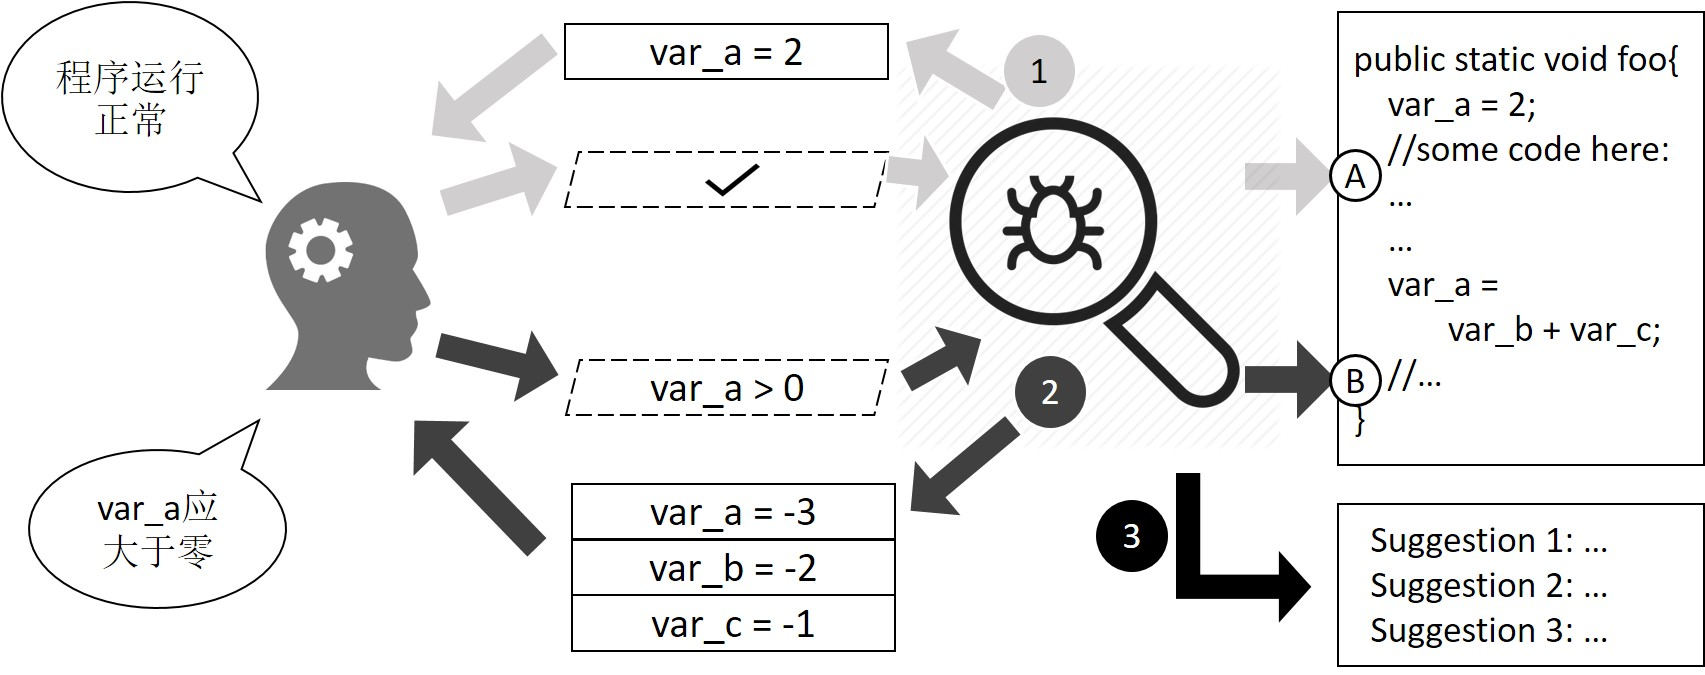
\includegraphics[width=1\linewidth]{chap04/interact-model}
	\caption{交互模式示意图}
	\label{fig:interact-model}
\end{figure}

在示意代码中,函数\texttt{foo}内部包含了几个变量\texttt{var\_a},\texttt{var\_b},\texttt{var\_c}。在一般的调试过程中,开发人员将在A点和B点各加一个断点。启动调试器(例如JDT Debugger)后,程序将首先暂停在A点,开发人员观察当前栈上的变量值,发现此时程序运行正常,因此恢复调试进程,程序继续运行。接着程序暂停在B点,此时开发人员发现变量\texttt{var\_a}的值为\texttt{-3},然而此时\texttt{var\_a}本应是正值,这说明在A点和B点之间程序运行出错,于是开发人员需要在两个断点之间再加入新的断点,逐步查找程序中的错误。

在上述调试过程中,开发人员在A点和B点对程序的运行状态进行判断,使得错误调试的范围缩小在两点之间。为利用这一判断,我们在现有“生成-检验”框架下设计了如下的交互模式:

\begin{enumerate}[1.]
	\item 开发人员根据对程序的初始判断,在认为与错误相关的地方加入断点
	\item 开发人员启动调试器,并判断断点处程序的运行状态是否正确。如果正确则标识“通过”(图\ref{fig:interact-model}中路线\textcircled{1}),否则输入对程序运行状态的期望描述,例如“\texttt{var\_a > 0}”(图\ref{fig:interact-model}中路线\textcircled{2})。系统将记录这一判断,生成带标注的“检查点”
	\item 开发人员选择一个状态不正确的检查点作为调试目标,系统搜索可能的修复方案,返回给开发人员(图\ref{fig:interact-model}中路线\textcircled{3})
	\item 如果系统在一定时间内没有返回合理的修复方案,则开发人员可增加更多的检查点,返回第2步
\end{enumerate}

上述交互模式综合了开发人员和系统在调试任务上各自的优势。一方面,开发人员对调试任务的先验知识可对“生成-检验”系统的错误定位结果起到补充作用。当程序错误比较复杂需要修改多处代码时,通过设置检查点可以将程序执行过程分解为小段,每小段中包含一处需要修改的代码,这样修复系统能够处理。另一方面,由于使用了“生成-检验”系统的修复方案自动生成功能,开发人员可以减少调试过程中“重启调试 $\rightarrow$ 单步跟踪”的次数。例如在图\ref{fig:interact-model}中,当发现B点程序运行出错时,不需要重启程序并退回到A点开始单步跟踪。

\subsection{系统结构}%1


\begin{figure}
	\centering
	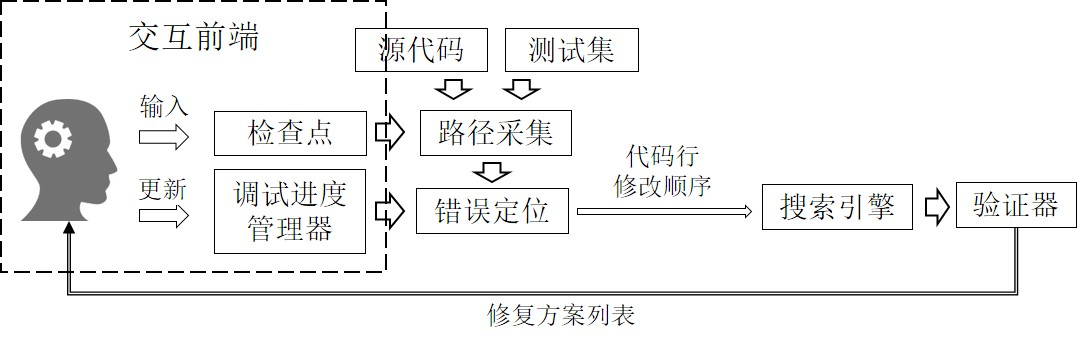
\includegraphics[width=1\linewidth]{chap04/sys-structure}
	\caption{系统结构示意图}
	\label{fig:sys-structure}
\end{figure}

图\ref{fig:sys-structure}展示了框架扩展后的系统结构。如图所示,在一般的“生成-检验”模块前,我们加入了一个“交互前端”,方便开发人员与后端的修复生成系统交互。
交互前端内部包含两个模块。一是检查点及其相关管理模块,负责接收用户对程序运行状态的判断。检查点具有以下属性:
\begin{itemize}
	\item 关联测试用例。被测程序的测试集通常包含多个测试用例,每个检查点最多关联一个测试用例
	\item 位置信息。即在某个测试用例执行过程中的一个特定位置,以代码行号和经过这一行的次数表示
	\item 执行状态信息,包括开发人员对程序运行到此处的状态的判断,“正确”或“不正确”,如不正确,还包含以一个合法Java布尔表达式描述的对程序运行状态期望。特殊的情况是,如果需要表示程序应该在每次经过该检查点所在的代码位置时都满足所输入的布尔表达式,那么应在位置信息的“次数”这一属性上填入“一直满足”
\end{itemize}

二是调试进度管理器,负责实时更新当前所有检查点的运行状态。在程序调试过程中,可能出现多个检查点运行状态都不正确的情况,此时用户可以在调试进度管理器中每次选择一个检查点作为调试目标,逐步修改程序以完成调试任务。

开发人员通过交互前端输入其对程序的先验知识,系统则根据这些信息调整搜索过程。原有框架中有两个模块的设计和实现需要调整,一是错误定位模块,其定位结果应依照检查点的状态有所改变,而是检验器,其检验标准应随调试目标的变化而变化。在以下两个小节中我们重点介绍这两个模块的调整方案。


\subsection{扩展的错误定位}%0.6

在原框架下,错误定位模块的输入是由路径采集模块记录的测试用例执行路径。定位算法采用SFL定位算法中的Ochiai\cite{Abreu:2006:ESC:1193217.1194368}算子,对每个代码行$l$,其出错的概率估计$sus_l$为:
$$sus_l = \frac{a_{ef}}{\sqrt{(a_{nf} + a_{ef}) (a_{ef} + a_{ep})}}$$
其中,$a_{ef}$表示经过该代码行且执行失败的测试用例数,$a_{ep}$表示经过该代码行且通过的测试用例数,$a_{nf}$表示未经过该代码行且通过的测试用例数。

在扩展框架下,定位算法应利用检查点的属性生成更精确的定位结果。在引入检查点后,一个未通过的测试用例对应的路径可能被检查点分成了很多段。精确地说,设一个未通过的测试用例$t_f$的测试路径为$L = {l_{1,1}, \dots,l_{1,m},cp_p, l_{u,1}, \dots ,l_{u,v}, cp_f}$,其中$cp_f$是第一个未通过的检查点,$cp_p$是$cp_f$前的最后一个检查点,那么我们知道在$L_1 = {l_{1,1}, \dots,l_{1,m}}$这段路径上程序运行正确,而在$L_2 = l_{u,1}, \dots ,l_{u,v}$这一段上必然有至少一处代码是错误的。因此,在统计SFL算子的输入时,路径$L$会被拆分为两条路径$L_1$和$L_2$,而错误定位模块最终输出的调试顺序列表也仅包含$L_2$中的代码行。由此,开发人员借助检查点圈定了错误存在的范围,系统在后续搜索过程中也可以节省时间。

\subsection{调试进度控制}%1.5


\begin{figure}[!b]
	\centering
	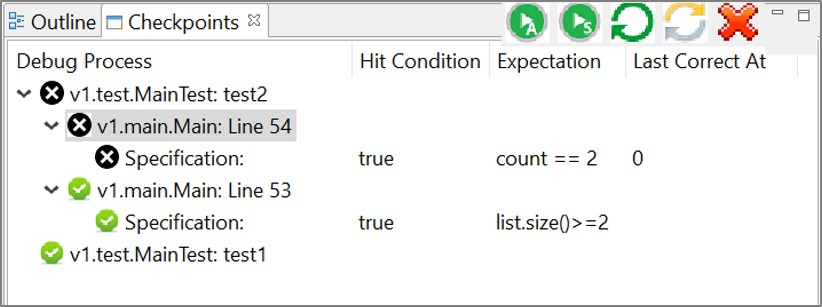
\includegraphics[width=0.7\linewidth]{chap04/progress-control}
	\caption{调试过程控制面板}
	\label{fig:progress-control}
\end{figure}

当被测程序错误比较复杂时,可能出现多个测试都未通过且程序需要修正的位置不止一处的情况。此时,开发人员可以为每个不通过的测试用例都加入一组检查点,逐一程序在检查点上的运行状态,从而将调试任务分解为几个子任务逐步解决。在解决任务的过程中,不同测试用例的检查点状态也不相同。系统为检查点规定了三种状态,“通过”,“不通过”和“未知”。其中,“通过”表示检查点所属的测试用例在这一位置上运行正确或在修复了某些错误后检查点上的“用户期望”表达式得到满足。相反的,“不通过”表示测试用例运行不正确,“用户期望”表达式未被满足。“未知”表示未对这一检查点做判断。

图\ref{fig:progress-control}展示了系统的调试进度控制面板,面板上列出了当前测试用例及其检查点的状态。每次对修改程序后,刷新控制面板,系统将自动执行所有测试用例,并判断检查点的状态,更新面板。这一功能实现在JDT Debug插件上,对每个测试用例,系统首先将每个检查点转化为JavaLineBreakpoint注册到JDT调试管理器中,同时实现一个断点监听器,在回调函数中判断检查点中的期望表达式是否被满足。接着以调试模式运行程序,在程序运行过程中,监听器会被触发,一旦某个检查点上程序没有通过,则标为“不通过”,之后未触发的检查点都标为“未知”。

在分步调试过程中,开发人员可以选择任何一个当前具有未通过检查点的测试用例作为调试对象。此时,调试的目标是使调试进程“前进一步”,即通过这个检查点。因此,后台系统的检验模块验证一个备选修复方案是否通过的标准将从“通过所有测试用例”变为,在保证其他已通过的检查点仍然通过的基础上,使被选中的测试至少多通过一个检查点。这样,程序错误将逐步修复。


\subsection{实验结果}%1
在PFDebug的基础上,我们将交互式调试引入“生成-检验”框架,并实现为一个Eclipse插件工具SmartDebug。为评价SmartDebug的实际使用效果,我们设计了如下的对比试验。

首先,我们记录了一次研究生一年级上机编程考试过程中25名同学解答一道考题的编程过程。参加考试的同学均使用Eclipse集成开发环境,我们在后台记录了程序的编辑历史,包括每次保存操作、调试操作对应的程序版本。考试结束后,我们恢复出开发过程中出错的版本作为被测程序。最后,我们邀请了20余名未参加考试的同年级同学参加SmartDebug的评价实验。参与人员随机分为两组,一组仅通过人工方式调试被测程序,一组使用SmartDebug辅助调试。我们记录了两组同学完成调试任务所需的时间并比较两种情况下的调试时间。

表\ref{tab:sd-vs-human}列出了实验结果。SmartDebug的搜索空间覆盖了25个错误版本中的8个,错误类型包括使用了错误的局部变量、循环变量、错误的操作符等。在这8个程序上,使用SmartDebug一般可以在5分钟以内完成程序修复。在7个版本上,借助SmartDebug的修复效率高于人工修复。其中值得注意的是,1号程序有两个错误,SmartDebug可以通过分段调试的方式分别解决两个问题。

以上实验结果表明,引入交互式调试模式的“生成-检验”系统能够对开发人员的调试工作起到一定的帮助作用。

\begin{table}[!t]
	\centering
	\caption{SmartDebug v.s. Human}
	\label{tab:sd-vs-human}
	\begin{tabular}{|c|l|c|c|} \hline
		序号& 错误简介 									& SD(s) & H(s)	\\	\hline
		1  & variable replacement \& operator change				& 282	& 300	\\	\hline
		2  & wrong operator									& 95	& 691	\\	\hline
		3  & wrong usage of a local variable				& 1055	& 694	\\  \hline
		4  & wrong usage of loop variables					& 260	& 423	\\	\hline
		5  & wrong usage of loop variables					& 309	& 410	\\	\hline
		6  & wrong usage of loop variables					& 198	& 341 	\\	\hline
		7 & wrong usage of a numeric variable				& 215	& 829	\\	\hline
		8 & wrong usage of a local variable				& 228	& 600	\\	\hline
		
	\end{tabular}
\end{table}

\section{针对单类别错误的可扩展框架}%12

\subsection{概述}%1

基于“生成-检验”框架的自动修复系统本身并不针对特定类型的错误修复程序,其能够修复的错误范围是由系统内部搜索引擎的搜索空间决定的。这种设计的优点是系统在理论上具有普适性,例如当程序中的错误来自软件的业务逻辑层而非底层实现时,系统仍有可能成功修复程序。但是,如上文中所分析的,目前“生成-检验”系统的搜索引擎能够负担的搜索空间比较小,很多实际程序中的错误都无法覆盖,这导致这一类系统投入实用还比较困难。

实现错误自动修复的另一条技术路线是针对特定类型的错误研究专门的修复方案。这一类工作通常针对较底层的错误,如空指针异常、数组越界、死锁、数据竞争等。这类错误在程序执行过程中表征明显,与软件本身的业务逻辑关系不大,分析算法也比较成熟,因此针对特定类型的错误修复算法容易做到准确、高效。

事实上,以上两种技术路线具有一定的互补性。前者不限制错误类型,但准确度和效率较低,后者性能较好但错误类型受限。由此,本文提出扩展“生成-检验”系统框架,使得针对特定类型错误的各类修复算法可以方便的集成到框架中,而在使用时开发人员可以根据具体情况选择所需的算法,则扩展系统可以兼具两种技术路线的优点。

为达成上述目标,框架扩展过程中需解决以下两个问题。第一,不同修复算法计算步骤各不相同,若将其统一在同一个框架中,则需在合适的粒度上规范各个算法的操作流程,使得各个算法具有规整的代码结构,但仍能有不同的功能实现。第二,为方便算法集成,应合理设计“生成-检验”系统各模块间的接口,将公用功能抽出,为其他算法提供较好的基础设施,尽量避免重复代码。

在本节中,我们从“生成-检验”框架的结构出发,分析针对特定类型错误的修复算法一般流程与“生成-检验”系统的计算流程的共同点,最终将不同修复算法以“子搜索引擎”方式集成在系统中。此外,我们将已有系统中路径收集模块、错误定位模块以及检验器模块的接口规范化,设计API,方便不同算法实现重用已有功能。最后,我们以一个空指针异常修复系统NPEDebug为例,说明了如何利用已有系统完成针对特定类型错误的修复算法定制开发。我们将NPEDebug用于修复CWE空指针引用(Null Pointer Dereference)类别下的6类测试用例,实验结果表明NPEDebug可以成功修复其中5类错误。这一结果证明了将针对特定类型修复算法融合进“生成-检验”框架的可行性。


\subsection{相关工作}%2

\subsubsection{针对特定类型错误的修复算法}

\textbf{空指针(Null Pointer)错误修复算法:}
\cite{Sinha:2009:FLR:1572272.1572291}提出了针对Java程序中的运行时异常的错误定位和修复算法,理论上其能够处理的异常类型包括空指针(NullPointerException)、算数运算(ArithmeticException)、类型错误(ArrayStoreException)。该算法将动态分析与静态后向数据流分析相结合,能够定位错误的赋值语句,同时也分析出该语句在不同运行场景下可能触发的其他异常。最终作者将该方法实现并应用于定位和修复空指针异常。\cite{DBLP:journals/corr/CornuDSM15}中,作者参考“生成-检验”框架中的“修复模板”概念,提出了修复空指针异常的9条修复模板,并通过在程序的执行过程中监控变量取值找出适合使用模板的程序位置,最终生成修复方案。

\textbf{数值错误:}工作\cite{Zhang2010}中,作者针对“整数溢出导致缓冲区溢出(IO2BO)”错误提出检测和修复算法,并实现工具IntPatch。IntPatch利用类型论和数据流分析框架检测可能的IO2BO错误,并能够在编译阶段在程序中插入运行时检查语句。此外,IntPatch为程序员提供了检查整数溢出错误的接口。实验表明,IntPatch能够成功捕捉到IO2BO错误,并且处理后的程序运行效率平均仅降低1\%。\cite{7551988}针对C程序中的整数缺陷提出修复方案。作者提出,许多整数缺陷可以通过适当增加整数变量的精度完成修复,并基于此开发了工具CIntFix。实验表明,CIntFix成功修复了Juliet测试集中来自7个缺陷类别的5414 programs,在SPEC CINT2000测试集上的处理速度达到了0.157s/千行代码,修复后的程序平均有18\%的效率损失。

%\textbf{字符串错误:}\cite{Dhar:2015:CSP:2786805.2786877}
%	author = {Dhar, Aritra and Purandare, Rahul and Dhawan, Mohan and Rangaswamy, Suresh},
%	title = {CLOTHO: Saving Programs from Malformed Strings and Incorrect String-handling},
	
%Software is susceptible to malformed data originating from untrusted sources. Occasionally the programming logic or constructs used are inappropriate to handle the varied constraints imposed by legal and well-formed data. Consequently, softwares may produce unexpected results or even crash. In this paper, we present CLOTHO, a novel hybrid approach that saves such softwares from crashing when failures originate from malformed strings or inappropriate handling of strings. CLOTHO statically analyses a program to identify statements that are vulnerable to failures related to associated string data. CLOTHO then generates patches that are likely to satisfy constraints on the data, and in case of failures produces program behavior which would be close to the expected. The precision of the patches is improved with the help of a dynamic analysis. We have implemented CLOTHO for the JAVA String API, and our evaluation based on several popular open-source libraries shows that CLOTHO generates patches that are semantically similar to the patches generated by the programmers in the later versions. Additionally, these patches are activated only when a failure is detected, and thus CLOTHO incurs no runtime overhead during normal execution, and negligible overhead in case of failures.


\textbf{数据结构错误:}\cite{Demsky:2003:ADR:949343.949314}针对关键数据结构应满足的规约提出了一种描述语言,并能够动态检测和修复程序中不满足规约属性的数据结构,使程序能够在数据结构受损时稳定运行。进一步地,文章\cite{Demsky:2006:IED:1146238.1146266}提出对数据结构规约条件的自动生成算法。算法利用不变式检测工具Daikon推断数据结构应满足的一致性条件,开发人员可泛化或精化这些条件以获得合理的数据结构规约。将上述工作结合,开发人员可以较容易的描述、检测和修复系统中的数据结构错误。

%\cite{NokhbehZaeem2010}针对Java

%Contracts and specifications have long been used in object-oriented design, programming and testing to enhance reliability before software deployment. However, the use of specifications in deployed software is commonly limited to runtime checking where assertions form a basis for detecting incorrect program states to terminate the erroneous executions. This paper presents a contract-based approach for data structure repair, which allows repairing erroneous executions in deployed software by repairing erroneous states. The key novelty is the support for rich behavioral specifications, such as those that relate pre-states with post-states of the method to accurately specify expected behavior and hence to enable precise repair. The approach is based on the view of a specification as a non-deterministic implementation, which may permit a high degree of non-determinism. The key insight is to use any correct state mutations by an otherwise erroneous execution to prune the non-determinism in the specification, thereby transmuting the specification to an implementation that does not incur a prohibitively high performance penalty. While invariants, pre-conditions and post-conditions could be provided in different modeling languages, we leverage the Alloy tool-set, specifically the Alloy language and the Alloy Analyzer for systematically repairing erroneous states. Four different algorithms are presented and implemented in our data structure repair framework. Experiments using complex specifications show the approach holds much promise in increasing software reliability.


%We have implemented this approach and applied it to three sizable benchmark programs: CTAS (an air-traffic control system), BIND (a widely-used Internet name server) and Freeciv (an interactive game). Our results indicate that (1) automatic constraint generation produces constraints that enable programs to execute successfully through data structure consistency errors, (2) compared to manual specification, automatic generation can produce more comprehensive sets of constraints that cover a larger range of data structure consistency properties, and (3) reviewing the properties is relatively straightforward and requires substantially less programmer effort than manual generation, primarily because it reduces the need to examine the program text to understand its operation and extract the relevant consistency constraints. Moreover, when evaluated by a hostile third party "Red Team" contracted to evaluate the effectiveness of the technique, our data structure inference and enforcement tools successfully prevented several otherwise fatal attacks.

与获取数据结构的形式化规约不同,\cite{Elkarablieh:2007:ARC:1321631.1321643}提出将程序中的Assert语句看做程序规约并给出相应的数据结构修复算法。其基本思想是,首先利用符号执行计算当Assert语句被满足时受损的数据结构所应满足的约束条件,接着搜索能够使数据结构满足约束条件的修改方式。实验表明通过动态修改数据结构内容,程序能够从错误状态恢复并稳定运行。受符号执行技术限制,该算法通常可以修复规模在几百个节点的数据结构。在\cite{Elkarablieh:2007:SSA:1297105.1297056}中,作者引入静态分析技术提高算法的规模并开发新的工具STARC。给定一个描述数据结构约束的Java谓词方法,STARC通过静态分析识别该方法用于遍历数据结构的成员域以及目标数据结构中成员变量之间的约束关系。在程序运行过程中,STARC执行该谓词方法识别受损的数据结构,接着在之前静态分析结果的指导下系统性的修改受损数据结构。实验表明改进的算法能够将处理的数据结构规模扩大到几万个节点。


%\textbf{并发错误修复:}

%\cite{Jin:2011:AAF:1993498.1993544}
%Fixing software bugs has always been an important and time-consuming process in software development. Fixing concurrency bugs has become especially critical in the multicore era. However, fixing concurrency bugs is challenging, in part due to non-deterministic failures and tricky parallel reasoning. Beyond correctly fixing the original problem in the software, a good patch should also avoid introducing new bugs, degrading performance unnecessarily, or damaging software readability. Existing tools cannot automate the whole fixing process and provide good-quality patches.

%We present AFix, a tool that automates the whole process of fixing one common type of concurrency bug: single-variable atomicity violations. AFix starts from the bug reports of existing bug-detection tools. It augments these with static analysis to construct a suitable patch for each bug report. It further tries to combine the patches of multiple bugs for better performance and code readability. Finally, AFix's run-time component provides testing customized for each patch. Our evaluation shows that patches automatically generated by AFix correctly eliminate six out of eight real-world bugs and significantly decrease the failure probability in the other two cases. AFix patches never introduce new bugs and usually have similar performance to manually-designed patches.

%\cite{Liu:2012:AAF:2337223.2337259}	author = {Liu, Peng and Zhang, Charles},	title = {Axis: Automatically Fixing Atomicity Violations Through Solving Control Constraints},
%Atomicity, a general correctness criteria in concurrency programs, is often violated in real-world applications. What is worse is that the violations are difficult to be fixed by the developers, which makes the automatic bug fixing techniques attractive solutions. The state of the art aims at automating the manual fixing process and can not provide any theoretical reasoning and guarantees. We provide an automatic approach that applies the well-studied control theory to guarantee the maximal preservation of the concurrency degree of the original code and no introduction of deadlocks. Under the hood, we reduce the problem of violation fixing to a constraint solving problem using the petri net model. Our evaluation on 13 subjects shows that the slowdown incurred by our patches is only 40\% of that of the state of the art. With the deadlock-free guarantee, our patches incur moderate overhead (around 10\%), which is a worthwhile cost for safety.

%\cite{Jin:2012:ACF:2387880.2387902}	author = {Jin, Guoliang and Zhang, Wei and Deng, Dongdong and Liblit, Ben and Lu, Shan},	title = {Automated Concurrency-bug Fixing}, 

%Concurrency bugs are widespread in multithreaded programs. Fixing them is time-consuming and error-prone. We present CFix, a system that automates the repair of concurrency bugs. CFix works with a wide variety of concurrency-bug detectors. For each failure-inducing interleaving reported by a bug detector, CFix first determines a combination of mutual-exclusion and order relationships that, once enforced, can prevent the buggy interleaving. CFix then uses static analysis and testing to determine where to insert what synchronization operations to force the desired mutual-exclusion and order relationships, with a best effort to avoid deadlocks and excessive performance losses. CFix also simplifies its own patches by merging fixes for related bugs.

%Evaluation using four different types of bug detectors and thirteen real-world concurrency-bug cases shows that CFix can successfully patch these cases without causing deadlocks or excessive performance degradation. Patches automatically generated by CFix are of similar quality to those manually written by developers.

%\cite{Liu:2014:GCF:2635868.2635881}	author = {Liu, Peng and Tripp, Omer and Zhang, Charles},	title = {Grail: Context-aware Fixing of Concurrency Bugs},
%Writing efficient synchronization for multithreaded programs is notoriously hard. The resulting code often contains subtle concurrency bugs. Even worse, many bug fixes introduce new bugs. A classic example, seen widely in practice, is deadlocks resulting from fixing of an atomicity violation. These complexities have motivated the development of automated fixing techniques. Current techniques generate fixes that are typically conservative, giving up on available parallelism. Moreover, some of the techniques cannot guarantee the correctness of a fix, and may introduce deadlocks similarly to manual fix, whereas techniques that ensure correctness do so at the expense of even greater performance loss. We present Grail, a novel fixing algorithm that departs from previous techniques by simultaneously providing both correctness and optimality guarantees. Grail synthesizes bug-free yet optimal lock-based synchronization. To achieve this, Grail builds an analysis model of the buggy code that is both contextual, distinguishing different aliasing contexts to ensure efficiency, and global, accounting for the entire synchronization behavior of the involved threads to ensure correctness. Evaluation of Grail on 12 bugs from popular codebases confirms its practical advantages, especially compared with existing techniques: Grail patches are, in general, >=40% more efficient than the patches produced by other techniques, and incur only 2% overhead.


%\cite{Khoshnood:2015:CCS:2771783.2771798}	author = {Khoshnood, Sepideh and Kusano, Markus and Wang, Chao},	title = {ConcBugAssist: Constraint Solving for Diagnosis and Repair of Concurrency Bugs},

%Programmers often have to spend a significant amount of time in- specting the software code and execution traces to identify the cause of a bug. For a multithreaded program, debugging is even more challenging due to the subtle interactions between threads and the often astronomical number of interleavings. In this work, we pro- pose a logical constraint based symbolic analysis method to aid in the diagnosis of concurrency bugs and to recommend repairs. Both diagnosis and repair are formulated as constraint solving prob- lems. Our method, by leveraging the power of satisfiability (SAT) solvers and a bounded model checker, performs a semantic analy- sis of the sequential computation as well as thread interactions. The constraint based analysis is designed for handling critical software with small to medium code size, but complex concurrency control, such as device drivers, implementations of synchronization proto- cols, and concurrent data structures. We have implemented our new method in a software tool and demonstrated its effectiveness in di- agnosing bugs in multithreaded C programs.

%\cite{Cai:2016:FDV:2884781.2884819}	author = {Cai, Yan and Cao, Lingwei},	title = {Fixing Deadlocks via Lock Pre-acquisitions},
%Manual deadlock fixing is error-prone and time-consuming. Existing generic approach (GA) simply inserts gate locks to fix deadlocks by serializing executions, which could introduce various new deadlocks and incur high runtime overhead. We propose a novel approach DFixer to fix deadlocks without introducing any new deadlocks by design. DFixer only selects one thread of a deadlock to pre-acquire a lock w together with another lock h, where before fixing, the deadlock occurs when the thread holds lock h and waits for lock w. As such, DFixer eliminates a hold-and-wait necessary condition, preventing the deadlock from occurring. The thread performing pre-acquisition is carefully selected such that no other synchronization exists in between the two original acquisitions. Otherwise, DFixer further introduces a context-aware conditional protected by above lock w to guarantee the correctness of DFixer. The evaluation is on 20 deadlocks, including 17 from widely-used real-world C/C++ programs. It shows that DFixer successfully fixed all deadlocks. Whereas GA introduced 9 new deadlocks; a latest work Grail failed to fix 8 deadlocks and introduced 3 new deadlocks on others. On average, DFixer incurred only 2.1% overhead, where GA and Grail incurred 15.8% and 11.5% overhead, respectively.


\subsection{框架设计}%4

图\ref{fig:extend-framework}展示了扩展的“生成-检验”框架。为设计合理的扩展框架,我们首先将原有框架整理,并抽出针对一般类型错误和特定类型错误的不同修复算法可重用的功能模块,以实线框图表示,包括与用户交互的“检查点”、“调试进度管理器”,负责处理路径信息的路径收集和错误定位模块,负责“生成”的搜索引擎框架和通用修复模板系统,提供搜索空间压缩的与过滤器以及负责“检验”的验证器。接着,我们分析上小节中提到的针对特定类型错误的算法设计思路,发现无论修复何种错误,均需经过“错误定位”和“修复生成”两个步骤。因此我们将第一个步骤对应的计算模块抽象为“特定类型错误分析器”,其计算结果将生成“特定类型错误修复位置”列表。将第二个步骤抽象为“定制修复模板系统”,封装不同的“特定类型错误修复算法”。最终,当需要在系统中添加新的错误定位算法时,只需实现一组图中灰色框图模块,与其他系统固有模块组合即可。

下面我们将详细介绍系统各模块所提供的的具体功能和可扩展接口。

\begin{figure}
	\centering
	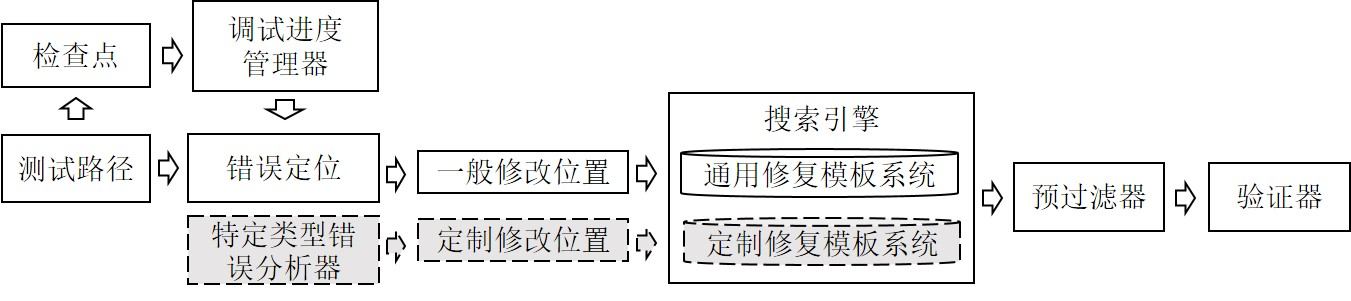
\includegraphics[width=1\linewidth]{chap04/extend-framework}
	\caption{扩展框架设计}
	\label{fig:extend-framework}
\end{figure}


\subsubsection{搜索引擎}

搜索引擎是扩展框架的核心部分,其功能是提供一个公用搜索流程控制接口,使得在实现针对不同类型错误的生成算法时只需关注针对某一特定位置的修复算法而不需重复编写整个流程控制代码。代码\ref{code:searchframe}展示了搜索引擎(\texttt{SearchEngine})实现的代码框架:


\begin{lstlisting}[caption=搜索框架,frame=single,language=Java,numbers=left,basicstyle=\ttfamily\footnotesize,label={code:searchframe},tabsize=2]
public class SearchEngine extends Job{

	private FixGenerator fixGenerator;
	private FixValidator fixValidator;
	private BugFixSession session;

	public SearchEngine(BugFixSession session, 
			FixGenerator fixGenerator){...}
	
	@Override
	protected IStatus run(IProgressMonitor monitor) {
		try {
			session.initFixSession();
			fixValidator = new FixValidator(session);
			fixGenerator.init();

			while(session.getBBProgress() < 
					session.getSuspectList().size()){
				
				for(int i = session.getBBProgress(); 
						i < allSuspiciousBlockNum; i ++){
					BasicBlock bb = session.getSuspectList().get(i);
					ArrayList<Fix> fixes = fixGenerator.searchFixes(bb);
					session.getCandidateQueue().appendNewFixes(fixes);
					session.increaseBBProgress();
					
					if(session.getCandidateQueue().getSize() > 30)
						break;
				}
								
				while(session.getCandidateQueue().hasNextFix()){
					Fix fix = session.getCandidateQueue().getNextFix();
					fixValidator.validate(fix);
				}
			}			
		} finally {
			monitor.done();
		}		
		return Status.OK_STATUS;
	}
	...
}
\end{lstlisting}

\texttt{SearchEngine}类包含了三个主要成员域,其类型是修复方案生成器\texttt{FixGenerator},修复方案验证器\texttt{FixValidator}以及修复会话\texttt{BugFixSession}。在初始化时,系统需指定所需的\texttt{FixGenerator}实例并将其传入。不同的FixGenerator实现对应不同的修复算法,其功能体现在搜索流程实现方法\texttt{run}中。

在\texttt{run}方法内部,首先初始化修复会话\texttt{session}(第13行),完成收集信息收集、利用SFL算法计算错误定位结果等操作,接着新建修复建议验证器(14行),调用\texttt{FixGenerator}的\texttt{init}接口完成修复建议生成器所需的初始化操作(15行)。此处的\texttt{init}是开放接口,由于此时修复会话内部的数据结构已经建立,不同的搜索算法可在此基础上完成各自所需的分析工作。搜索流程的核心结构是,对错误定位结果列表中的所有基本块上逐组完成“生成”和“检验”两个计算步骤(第20-34行\texttt{while}循环)。循环内部分为两个步骤,第一是生成修复方案(第20-28行)并将其添加到候选方案列表中,其中调用了\texttt{FixGenerator}的修复方案生成接口\texttt{searchFixes(BasicBlock bb)},用于封装不同修复算法的具体实现。第二是利用\texttt{FixValidator}提供的\texttt{validate}方法逐个验证候选方案列表中的修复方案是否满足要求(第31-34)行。为保证修复生成与检验的进度平衡,在候选修复建议超过30条时,搜索过程将从“生成”转向“检验”(第27-28行),这是由于“检验”通常比较耗时,在正确的修复方案出现后应尽早将其检验并返回给使用者。

代码\ref{code:searchframe}中省略了两个细节。第一,\texttt{SearchEngine}继承自Eclipse的“任务”\texttt{Job}类,\texttt{run}方法是重写方法,方法内部利用类\texttt{IProgressMonitor}实现了搜索进度的控制与界面展示,方便使用者了解算法的运行进度。第二,计算过程中可利用系统提供的日志管理器打印日志,在开发过程中了解系统的执行过程,方便调试。

不同类型修复算法均需使用上述搜索框架,框架内涉及到的开放接口或系统模块包括修复会话(\texttt{BugFixSession}),修复生成器(\texttt{FixGenerator})以及修复验证器\texttt{FixValidator}。以下将详细介绍三个类的使用方式。

\subsubsection{修复会话(BugFixSession)}%0.5p
修复会话表示“一次修复方案计算过程”,在类\texttt{BugFixSession}内部包含此次计算过程所需的基本数据。

数据分为三类:
\begin{itemize}
	\item 修复任务的基本信息,包括被测程序、测试集、每个测试用例的测试结果。在原有系统框架中,被测程序是Eclipse中的一个Java工程(Project)对象,测试集是一组JUnit测试方法集合,测试结果则是JUnit测试结果,包括通过/不通过,以及不通过时错误方法调用栈。这类信息在\texttt{BugFixSession}初始化时完成收集
	\item 根据基本信息产生的一些分析结果,包括测试用例的覆盖情况以及SFL算法据此计算出的初始错误定位排序结果。
	\item 与使用者交互相关信息,包括修复算法的选择,即具体使用了哪一类修复修复方案生成器,用户添加的检查点、各个检查点的当前状态、用户此次选择的修复目标。系统向不同修复算法开放这部分功能,方便实现过程中缩小错误定位范围,提高系统效率,也增加与使用者的交互性。
\end{itemize}

以上三类信息均对搜索引擎的搜索过程起到指导作用,因此均提供了开放接口以供其他模块查询。

\subsubsection{修复生成器(FixGenerator)}%1p

修复生成器封装了针对不同错误修复算法的具体实现。框架将各修复算法的计算步骤抽象为两步,一是根据测试过程中产生的数据分析错误的原因,对应原框架中的“错误定位”,二是根据错误定位的结果针对每个可能出错的位置生成“修复方案”,对应原框架中搜索引擎中预置的“搜索模板”。不同算法在这两步的具体实现不同,但为嵌入整体框架,算法需继承\texttt{FixGenerator}类,并将两个步骤的算法封装在以下两个接口中:

\begin{lstlisting}[frame=single,language=Java,basicstyle=\ttfamily\footnotesize,tabsize=2]
public void init();
\end{lstlisting}

\texttt{init}方法对应“错误定位”部分,参照它在\texttt{SearchEngine}中被调用的位置,可以看出此时\texttt{BugFixSession}已经完成了基本的信息收集,也有了初步的定位结果,若不同算法内部还需根据这些信息做进一步的分析计算,则可在\texttt{init}方法中完成,实现特定算法\texttt{FixGenerator}的初始化。

\begin{lstlisting}[frame=single,language=Java,basicstyle=\ttfamily\footnotesize,tabsize=2]
public ArrayList<Fix> searchFixes(BasicBlock bb);
\end{lstlisting}

\texttt{searchFixes}方法针对一个具体的修复位置产生修复方案。其中输入参数\texttt{BasicBlock}是原有框架中表示Java代码基本块的数据结构。该结构中包含了基本块所在的代码文件、文件行号和具体代码内容。返回类型是\texttt{ArrayList<Fix>}是一组对应该修改位置的修复方案,其中\texttt{Fix}是系统中所有修复方案的抽象类型,具体细节在下一节介绍。

在实现上述接口后,\texttt{FixGenerator}的不同实现均可无缝嵌入搜索引擎。

\subsubsection{检验器(FixValidator)}%0.4p
检验器的功能是将修复方案应用回源代码,重新编译并运行测试集,检验修复方案是否能够完成本次修复会话的修复目标。系统提供了完整的检验器功能实现,新加入的算法可直接利用这一功能。但由于不同算法生成的修复方案也不相同,为利用已有检验器功能,所有修复方案都应继承自类\texttt{Fix}并实现以下三个接口:

\begin{lstlisting}[frame=single,language=Java,basicstyle=\ttfamily\footnotesize,tabsize=2]
public void doFix();
public void undoFix();
public IFile[] getModifiedFiles();
\end{lstlisting}

在检验过程中,\texttt{FixValidator}首先调用修复方案的\texttt{doFix}方法完成对源代码的修改操作,接着调用\texttt{getModifiedFiles()}查看被修改的文件列表,编译程序并判断是否有编译错误,如果没有则重新运行测试查看结果。若通过检验,修复方案将被添加到修复方案列表中提交给使用者。最后,\texttt{FixValidator}调用\texttt{undoFix()}还原源代码。

三个接口的具体实现通常需要调用Eclipse代码操作API,原有系统中已有示例实现可供参考。

\subsubsection{其他公用设施}%1p
系统提供了一些其他公共设施方便新算法的实现。首先是表达式生成器\texttt{ExpressionGenerator},此类实现了在不同上下文中生成符合要求的表达式集合的多种方法,包括生成可替换If条件的布尔表达式、替换特定语法类型的一般表达式,根据目标表达式所在的代码位置获取局部变量、同类成员域、静态成员域,将不同表达式以运算符、方法调用等方式结合起来生成复合表达式等。生成方法实现在Eclipse AST上,因此输入参数也是AST中的元素。

第二是第三章“预过滤”策略的封装。算法生成的修复方案需要利用预过滤策略对搜索空间剪枝,则首先修复方案应继承自\texttt{FilterableFix}类并实现其中的相应接口。\texttt{FilterableFix}扩展了类\texttt{Fix},增加的主要成员域是“目标表达式”与“替换表达式”。将修复方案转化为\texttt{FilterableFix}的方案可参见第三章表\ref{tab:search-space}。需要注意的是,搜索引擎并没有主动调用预过滤器,这是由于不同算法对预过滤器的需求不同,因此各个算法应在\texttt{FixGenerator}的\texttt{generateFix}方法中完成预过滤,将最终结果返回给\texttt{SearchEngine}。

最后,为方便算法开发与调试过程,系统提供了一个公用的日志生成器\texttt{Logger},其提供的打印日志接口是:
\begin{lstlisting}[frame=single,language=Java,basicstyle=\ttfamily\footnotesize,tabsize=2]
public void log(int mode, String cause, String info);
\end{lstlisting}

其中,\texttt{mode}表示日志条目类型,\texttt{cause}表示记录事件类型,\texttt{info}表示日志信息。该方法会将上述信息按照统一格式整齐打印,并添加时间戳。

\subsection{扩展示例}
Java语言中空指针异常(NullPointerException,简称NPE)是一种常见的运行时异常。当异常意外触发而没有合适的捕获处理机制时,该异常将导致程序执行中断,无法完成任务。针对NPE常见的修复方式是在合适位置提前加入空指针检查,或在空指针解引用操作出现时提供合适的非空对象。\cite{DBLP:journals/corr/CornuDSM15}中,作者提出了9条修复模板,事实上也分别属于这两类操作。在本节,我们在扩展框架上以实现针对空指针异常的修复系统NPEDebug为例,说明扩展框架二次开发的基本方法。

在扩展框架中实现针对特定类型的修复系统,基本想法是尽量利用系统中的已有功能快速开发,同时通过引入对特定错误的分析算法提高错误定位精度和修复方案生成准确度,提高系统效率。在NPE异常修复中,我们首先利用反向切片算法进一步缩小错误范围,接着定制搜索引擎中的错误生成模板,缩小搜索空间,从而达到较好的修复效果。

\subsubsection{NPEFixGenerator}

类\texttt{NPEFixGenerator}是NPEDebug系统中针对空指针异常定制的修复方案生成器,按照系统框架的要求,该类需实现\texttt{init}与\texttt{generate}两个方法,分别用于初始化和生成修复方案。

在\texttt{init}方法中,\texttt{NPEFixGenerator}根据异常信息定位触发异常的位置,并使用反向切片技术分离代码中与异常触发相关的程序语句,将其保存。其中,反向切片是通过调用Wala分析框架中的BackwardSlicing接口完成的。进行这一操作的原因是,原有系统给出的错误定位算法,其代码排序的基本单位是“基本块(Basic Block)”,即在任意执行路径上都会同时执行的代码语句组合。同一基本块中的语句虽然会同时执行,但语句之间并不存在必然的控制流与数据流依赖关系。若完全按照这一错误定位结果生成修复方案,则可能会在“执行了”但“与异常触发”无关的语句上浪费搜索时间。因此将后向切片结果与SFL算法结果相结合,可以得到所有与NPE异常触发相关语句的合理优先级排序结果。

参考系统中针对一般类型错误的修改生成器实现,在获得反向切片结果后,\texttt{NPEFixGenerator}借助类\texttt{NPEFixSiteManager}存储切片结果、管理与NPE相关语句所在位置。在\texttt{searchFixes()}方法中,\texttt{NPEFixGenerator}首先根据输入的\texttt{BasicBlock}对象,在\texttt{NPEFixSiteManager}中查找相关的程序语句,接着分析可能存在空指针解引用操作的表达式,并使用针对NPE的修复模板生成修复方案。这里使用的修复模板分为两类,一类是空指针检查,一类是为空值对象赋值。具体的修复模板以及使用预过滤算法的方式参见表\ref{tab:npe-search-space}。

\begin{table}
	\centering
	\caption{NPE修复模板系统}
	\label{tab:npe-search-space}
	\begin{tabular}{|p{1.3cm}|p{6cm}|p{2.5cm}|p{1.2cm}|p{1.7cm}|}
		\hline
		修复模板                & 含义         & 搜索空间说明 & $e_t$ & $e_r$                                    \\ \hline
		
		引入新分支			& 插入\texttt{if(obj == null) return/break/continue;}
		& obj是下文将解引用的对象		&\texttt{false}  & \texttt{obj == null}				\\ \hline		
	
		空指针检查      & 	插入\texttt{if(obj != null)\{ visit(obj);\}}
		& obj是下文将解引用的对象		&\texttt{true}	&\texttt{obj != null}		 \\ \hline
		
		空值变量赋值      & 	插入\texttt{if(obj == null)\{ obj = $e'$\}}
		& obj是下文将解引用的对象  	&\texttt{false}	&\texttt{obj == null}		 \\ \hline
		
	\end{tabular}
\end{table}

\subsubsection{NPEFix}%0.3
\texttt{NPEFixGenerator}生成出的修复方案类型为\texttt{NPEFix},继承自\texttt{FilterableFix}。依照框架规定,\texttt{NPEFix}需实现\texttt{doFix},\texttt{undoFix}和\texttt{getModifiedFiles()}三个接口。
扩展框架没有限定上述方法的具体实现方案,但提供了示例代码可供参考。在实际开发过程中,NPEFix直接调用了父类\texttt{FilterableFix}的实现。因此这里我们简单解释原系统中这几个函数的实现方式。

Eclipse平台提供了对Java工程 、包、文件等的封装结构和操作API。修复方案影响到的被修改文件是在生成过程中记录的。\texttt{doFix}和\texttt{undoFix}利用其中的文件操作API,将修复方案中对代码的修改方案实现为Eclispe代码编辑框架中的一个\texttt{TextEdit},并利用其自带的\texttt{apply}操作完成代码编辑,同时获取反向操作的编辑对象。



\subsubsection{NPEDebug实验}%1
为检验NPEDebug的实际应用效果,我们在CWE Juliet测试集中的Null Pointer Dereference类测试程序上对NPEDebug进行测试。测试集共包含375个测试用例,表\ref{tab:cwenpd}列出了测试集的基本信息。
\begin{table}
	\centering
	\caption{CWENPD测试集}
	\label{tab:cwenpd}
	\begin{tabular}{|l|l|l|}
		\hline
		类型                     & 数量 & 说明                         \\ \hline
		binary if              & 17 & 在if判断条件中应使用\&\&阻断右端表达式的NPD \\ \hline
		deref after check      & 17 & 在判断对象是空值后仍然访问对象            \\ \hline
		int array              & 81 & 访问空值数组                     \\ \hline
		Integer                & 81 & 访问空值整数                     \\ \hline
		null check after deref & 17 & 在访问对象后进行空值检查               \\ \hline
		String                 & 81 & 访问空值字符串                    \\ \hline
		StringBuilder          & 81 & 访问空值字符构造器                  \\ \hline
	\end{tabular}
\end{table}

测试用例错误可分为六类,其中“null check after deref”并不会导致程序崩溃,因此NPEDebug无法生成修复方案。对于其余的5类错误,NPEDebug可以生成有效的空指针检查语句,使得程序避开空指针异常正常执行。但对于第1类错误,NPEDebug无法生成最简单的修复方案。

\begin{lstlisting}[caption=CWE476\_NULL\_Pointer\_Dereference\_\_binary\_if\_12.java,frame=single,language=Java,numbers=left,basicstyle=\ttfamily\footnotesize,label={code:binary-if},tabsize=2]
public void bad() throws Throwable
{	
	if (IO.staticReturnsTrueOrFalse())
	{
		{
			String myString = null;
			/* FLAW: Using a single & in the if statement 
				will cause both sides of the expression to be
				evaluated thus causing a NPD */
			if ((myString != null) & (myString.length() > 0))
			{
				IO.writeLine("The string length is greater than 0");
			}
		}
	}
	else { ... }
}
\end{lstlisting}

代码\ref{code:binary-if}展示了其中一个binary-if错误示例。在代码第10行的if条件中,中间使用的\&符号应改为\&\&符号,从而使右端表达式在左端为空时不再计算。NPEDebug生成的修复方案是在\texttt{if}语句整体包裹在一个对\texttt{myString}做空指针检查的语句内部。这样固然可以使程序避开空指针异常,但是并不是最佳的解决办法。

一种可能的解决方案是扩展NPEDebug的搜索空间,增加对If条件表达式的修改。这可以覆盖这一类NPD错误,但程序的运行速度也必然有一定程度的下降。考虑到目前NPEDebug生成的修复方案可以使程序避免空指针异常,也比较容易理解,因此暂时保持了目前的系统版本。

\section{本章小结}%0.5

在本章中,我们分析了现有“生成-检验”修复框架存在的缺陷,并对此提出了两种框架扩展方案。
第一种是“交互式调试”模式扩展,通过为使用者提供接口描述对程序状态的判断,使得系统能够利用开发人员对程序的理解,提高错误定位的精度,从而提高系统的整体效率。在实验中,我们比较了人工调试与用系统辅助调试完成调试任务所需时间,结果表明,系统辅助调试所耗时间小于人工调试时间,这说明系统确实能够提高调试效率。

第二种扩展方案是规范现有框架中的模块功能与接口,使“生成-检验”系统成为能够融合针对特定类别错误的修复算法的可扩展框架。本章描述了框架设计,并在扩展框架结构上实现了针对空指针异常的修复系统NPEDebug。实验表明,NPEDebug能够修复CWE空指针解引用类别下的测试程序。




















